\section{Diseño experimental}
\subsection{Asunciones}
En este trabajo se tomarán como ciertos los siguientes puntos:
\begin{enumerate}
	\item Los conjuntos de datos elegidos se encuetran etiquetados correctamente 
	\item Cada imagen de los conjuntos de datos con los que se entrenarán los modelos resultan representativas a la escena a la que pertenecen.
	\item El hardware con el que se llevará a cabo el proyecto funcionará tal y como se establece en sus respectivo manual.
	\item Las redes preentrenadas a descargar, PlacesCNN e ImagenetCNN, fueron entrenadas sólo con las imágenes de los conjuntos datos Places365 e ImageNet, respectivamente.
	\item Para ambientes productivos la métrica exactitud categórica \cite{balanced_accuracy_score} es la más representativa.
\end{enumerate}

\subsection{Limitaciones} \label{ssec:limitaciones}
El proyecto en curso contará con las siguientes limitaciones:
\begin{enumerate}
	\item El análisis se centrará en imágenes de las siguientes escenas de propiedades: cocina, comedor, baño, dormitorio, exterior y living.
	\item Tanto los tiempos de entrenamiento y predicción como el tamaño de las redes, estarán restringidos al hardware con el que se cuenta.
	\item El trabajo intentará aceptar o refutar las hipótesis enumeradas a continuación, quedando excluídas del alcance del proyecto las posibles investigaciones que surjan a partir del mismo.
\end{enumerate}

\subsection{Hardware a utilizar} \label{ssec:hardware}
Para llevar adelante el trabajo se utilizarán los siguientes componentes:
\begin{itemize}
	\item Procesador Intel i7 de séptima generación versión U.
	\item Memoria RAM de 16gb.
	\item Disco sólido 256GB NVMe™ M.2 SSD.
	\item Tarjeta gráfica Gigabyte GTX 1080 de 8gb.
	\item eGPU HP Omen Accelerator.
\end{itemize}

\subsection{Hipótesis}
Teniendo en cuenta tanto las limitaciones como las asunciones definidas para el trabajo, se comprobarán las hipótesis declaradas a continuación. 

\subsubsection{Hipótesis 1} \label{sssec:hipotesis1}
Como se pudo observar en la revisión de antecedentes, existen múltiples formas de hacer frente al problema. El enfoque más simple podría ser mediante perceptrón multicapa, pero por lo que se pudo observar, la mayoría de las soluciones utilizadas son redes neuronales convolucionales. 

Hipótesis: "Una red convolucional es capaz de obtener mejores resultados que un perceptrón multicapa en materia de clasificación de escenas".

\subsubsection{Hipótesis 2} \label{sssec:hipotesis2}
Las redes convolucionales tienen la capacidad de aprender características de las imágenes con las que se entrenan, aunque a veces resulta muy costoso hacerlo por las diferencias entre imágenes de la misma categoría o bien no se cuenta con la cantidad de imágenes que aporten la densidad y diversidad necesaria para alcanzar el tope máximo en la métrica elegida. 

Hipótesis: "Una red convolucional obtendrá mejores resultados sobre un conjunto de test \(y\) siendo entrenada con conjunto de entrenamiento \(X\) que si es entrenada sólo con subconjuntos de 10\% o 50\% del conjunto de entrenamiento \(X\), respectivamente".

%\subsubsection{Hipótesis 3} \label{sssec:hipotesis3}
%Dado que la cantidad de escenas a clasificar es relativamente baja, sería posible plantear un enfoque en el que se entrene una red convolucional para cada una de las mismas. En este caso se trataría de clasificación binaria en la que la red sea capaz de detectar si se trata de una escena o no, aunque se debería tener en consideración el hecho de no estar cometiendo sobreentrenamiento. La hipótesis a analizar en este punto es: \(N\) redes convolucionales entrenadas como clasificadores binarios (una para cada escena) mejoran los resultados que utilizar una sola red convolucional para clasificar las mismas \(N\) clases, es decir, los resultados obtenidos de contrastar la hipótesis \ref{sssec:hipotesis2}.

\subsubsection{Hipótesis 3} \label{sssec:hipotesis3}
Como se pudo ver en \cite{learning_deep_features}, Zhou y otros crearon una red entrenada con millones de imágenes de escenas (Places Dataset) que debería ser capaz de predecir las imágenes de las escenas con las que fue entrenada. En términos de cantidad de imágenes, esta red está mucho más entrenada que las utilizadas en este trabajo. 

Hipótesis: "Realizar inferencia directamente a partir de esta red preentrenada alcanza mejores resultados que una red convolucional entrenada con el conjunto de datos del trabajo \cite{vision_based_real_estate_price_estimation} (el de mayor cantidad de imágenes que se tiene) para los conjuntos de validación y verificación definidos al contrastar la hipótesis \ref{sssec:hipotesis2}".

\subsubsection{Hipótesis 4} \label{sssec:hipotesis4}
Una de las técnicas revisadas antes de comenzar con el trabajo fue Aprendizaje por Transferencia (\ref{ssec:transfer_learning}), en el cual se parte de redes preentrenadas y se las reentrena con el conjunto de imágenes propio para ajustar los pesos de la red al mismo. 

Hipótesis: "Haciendo Aprendizaje por Transferencia a partir de la red PlacesCNN es posible mejorar los resultados obtenidos al contrastar la hipótesis \ref{sssec:hipotesis2}".


\subsubsection{Hipótesis 5} \label{sssec:hipotesis5}
Otra red pre-entrenada existente es ImageNetCNN, la cual fue entrenada con el dataset ImageNet centrado en objetos. Aunque no fue entrenada para escenas como PlacesCNN, se puede interpretar que tiene cierta capacidad de detectarlas a partir de los objetos que se encuentren en ella. 

Hipótesis: "La realización de Aprendizaje por Transferencia a partir de la red ImageNetCNN posibilita mejorar los resultados obtenidos al contrastar la hipótesis \ref{sssec:hipotesis2}".

\subsubsection{Hipótesis 6} \label{sssec:hipotesis6}
Un caso observado en la revisión de antecedentes es el de \cite{lstm_real_estate} en el cual se obtienen mejoras luego de aplicar un filtro de ecualización del histograma a las imágenes tanto para entrenar como para predecir. 

Hipótesis: "Realizar aprendizaje por transferencia utilizando PlacesCNN sobre un nuevo conjunto de datos obtenido a partir de aplicar el filtro utiizado en \cite{lstm_real_estate} para el conjunto de datos completo hará que los resultados sean mejores".

%\subsubsection{Hipótesis 7} \label{sssec:hipotesis7}

%Hipótesis: "Entrenar una red con la misma arquitectura que se entrenó para la hipótesis \ref{sssec:hipotesis2} pero utilizando un nuevo conjunto de datos obtenido aplicando el filtro utiizado en \cite{lstm_real_estate} para todo el conjunto de datos hará que se obtengan mejores resultados a los obtenidos al verificar la hipótesis \ref{sssec:hipotesis2}".

%\subsubsection{Hipótesis 8} \label{sssec:hipotesis8}
%La red ImageNetCNN fue entrenanda para detectar cientos de objetos diferentes, aunque en el caso de las escenas de propiedades inmuebles sólo un subconjunto de éstos son posibles de encontrar.

%Hipótesis: "Realizar aprendizaje por transferencia a partir de una versión reentrenada de la red ImageNetCNN con objetos posibles de encontrar en el contexto de las escenas de propiedades inmuebles hará que se obtengan mejores resultados a los obtenidos en el resto de los experimentos".


%\subsubsection{Hipótesis 7} \label{sssec:hipotesis7}
%Si se tiene en cuenta la cantidad de imágenes con el que se entrenó PlacesCNN y el conjunto de datos utilizado en el trabajo la diferencia es abrupta. Una manera de lidiar con la falta de datos es realizar Aumentación de los Datos.

%Hipótesis: "Hacer Aprendizaje por Transferencia partiendo de la red PlacesCNN pero realizando técnicas de Aumentación de Datos hará que los resultados obtenidos en el experimento realizado al contrastar la hipótesis \ref{sssec:hipotesis4} mejoren".



\subsection{Experimentos}
%Se validará cada hipótesis a partir de experimentos individuales con el fin de constratar cada una. 
Los conjuntos de datos a utilizar en los experimentos serán los generados en los trabajos \cite{vision_based_real_estate_price_estimation} y \cite{lstm_real_estate}, de los cuales se seleccionarán las escenas determinadas en las limitaciones del trabajo. En las tablas \ref{exp:distribution_rei} y \ref{exp:distribution_vision_based} se puede observar la distribución de escenas que contienen de los mismos. La métrica con la que se compararán los diferentes resultados será Precisión Categórica.

\begin{table}[h!]
	\centering
	\begin{tabular}{| l | r | }
		\toprule
		Escena &  Cantidad de imagenes \\
		\midrule
		backyard &       745 \\
		bathroom &       793 \\
		bedroom &      1593 \\
		frontyard &       884 \\
		kitchen &       992 \\
		living\_room &       852 \\
		\bottomrule
	\end{tabular}
	\caption{Imágenes por escena - Conjunto de datos del trabajo \cite{lstm_real_estate}}
	\label{exp:distribution_rei}
\end{table}

\begin{table}[h!]
	\centering
	\begin{tabular}{| l | r | }
		\toprule
		Escena &  Cantidad de imágenes \\
		\midrule
		bathroom & 10058 \\
		bedroom & 24123 \\
		dining\_room & 19500 \\
		frontyard & 24869 \\
		kitchen & 24234 \\
		living\_room & 24210 \\
		\bottomrule
	\end{tabular}
	\caption{Imágenes por escena - 	Conjunto de datos del trabajo \cite{vision_based_real_estate_price_estimation}}
	\label{exp:distribution_vision_based}
\end{table}

\subsubsection{Experimento 1} \label{sssec:exp1}
Se entranará tanto una red convolucional como un perceptrón multicapa con las imágenes del conjunto de datos generado en el trabajo \cite{vision_based_real_estate_price_estimation}. A continuación podremos comparar los resultados de ambos modelos de manera que será posible contrastarlos con la hipótesis \ref{sssec:hipotesis1}.

El perceptrón multicapa del experimento cuenta con cinco capas ocultas totalmente conectadas de 1024, 1024, 512, 256 y 128 neuronas en cada una, con una capa de dropout intercalada luego de cada una de ellas con probabilidad de 0.3, finalmente, una capa de salida con activación softmax como se observa en en anexo \ref{ssec:anexo4}.


Por el lado de la red neuronal convolucional se utilizará una arquitectura que concatenará dos bloques compuestos por: capa convolucional, capa de normalización en lote, capa convolucional, capa de normalización en lote, capa de pooling y capa de dropout; en el primer bloque las capas convolutivas aplicarán 64 filtros cada una, mientras que en el segundo 128, todos ellos de tamaño \([5\;x\;5]\) en todas las capas convolutivas, las capas de pooling aplicarán filtros de \([2\;x\;2]\) y las capas de dropout tendrán asignada una probabilidad de 0.25. Luego de estos bloques, la red seguirá con una capa totalmente conectada de 512 neuronas con regularización L2, una capa dropout con probabilidad 0.5 y la capa de salida con activación Softmax. La inicialización de los pesos de la red se realizará mediante inicialización de Xavier \cite{glorot2010understanding}. En \ref{ssec:anexo5} se puede observar la arquitectura de esta red.

En ambas redes se utilizaron de la misma manera las siguientes configuraciones: 
\begin{itemize}
	\item Tamaño del lote: la cantidad de imágenes a computar antes de realizar una actualización de pesos es de 64.
	\item Entradas: ambas redes se entrenaron con los tres canales de las imágenes (Red, Green, Blue), redimensionando cada una a \(128\; x\; 128\) y luego normalizando el valor de los colores (se divide el valor de cada pixel sobre 255, el valor máximo en la escala RGB).
	\item Optimizador: exactitud categórica. En cada lote contabiliza las veces en las que la posición de la probabilidad más alta se condice con la posición de la predicción correcta. Vale aclarar que los resultados, al utilizar una capa de activación softmax son \(one-hot\; encoders\), es decir, para cada imagen se tiene como resultado un vector de longitud igual a la cantidad de clases a predecir con la probabilidad para cada clase. 
	\item Función de pérdida: entropía cruzada categórica pesada por clase definida en  \ref{formula:custom_loss_function}.
\end{itemize}

Se llevó a cabo el entrenamiento de ambas redes con una porción de 4671 imágenes, guardando N para validación y N para verificación. Los resultados se pueden observar en la tabla \ref{exp1:results}.

\begin{table}[h!]
	\centering
	\begin{tabular}{| l | r | r |}
		\toprule
		Modelo entrenado & Exactitud Categórica &  Exactitud Categórica \\
		{} & Conj. de Validación &  Conj. de Verificación \\
		\midrule
		Perceptrón Multi-Capa & 0.114 & 0.145 \\
		Red Neuronal Convolucional & 0.826 & 0.826\\
		\bottomrule
	\end{tabular}
	\caption{Exactitud categórica por modelo para los conjuntos de validación y verificación experimento \ref{sssec:exp1}}
	\label{exp1:results}
\end{table}


A partir de los resultados expuestos en la tabla previamente mencionada, no se cuenta con las evidencias necesarias para negar la hipótesis \ref{sssec:hipotesis1}. 

\subsubsection{Experimento 2} \label{sssec:exp2}
Se entrenará la misma red que en \ref{sssec:exp1} pero esta vez con diferentes subconjuntos del conjunto de datos del trabajo \cite{vision_based_real_estate_price_estimation} y finalmente con el conjunto de datos completo. A partir de los resultados obtenidos será posible contrastar la hipótesis \ref{sssec:hipotesis2}.

En este experimento se utilizará la misma red neuronal convolucional detallada en el experimento \ref{sssec:exp1}, será entrenada con subconjuntos aleatorios tanto del diez como del cincuenta por ciento del conjunto de datos total elegido, además del entrenamiento con la totalidad del mismo. En la tabla \ref{exp2:distribucion_clase_datasets} se puede observar la cantidad de imágenes de cada clase que se tienen para cada el entrenamiento en cada experimento. Además, en la tabla \ref{exp2:distribucion_clase_datasets_validation_test} se muestran las distribuciones de los conjuntos de datos de validación y verificación por clase, que serán fijos para hacer posible el testeo correcto de la hipótesis.

\begin{table}[h!]
	\centering
	\begin{tabular}{| r | l | r |}
		\toprule
		Porcentaje & Escena &  Cantidad \\
		subconjunto & {} &  de Imágenes \\
		\midrule
		10 &     bathroom &       877 \\
		10 &      bedroom &      2067 \\
		10 &  dining\_room &      1662 \\
		10 &    frontyard &      2129 \\
		10 &      kitchen &      2074 \\
		10 &  living\_room &      2084 \\
		\midrule
		50 &     bathroom &      3588 \\
		50 &      bedroom &      8513 \\
		50 &  dining\_room &      6897 \\
		50 &    frontyard &      8748 \\
		50 &      kitchen &      8620 \\
		50 &  living\_room &      8607 \\
		\midrule
		100 &     bathroom &      9088 \\
		100 &      bedroom &     21710 \\
		100 &  dining\_room &     17534 \\
		100 &    frontyard &     22359 \\
		100 &      kitchen &     21848 \\
		100 &  living\_room &     21822 \\
		\bottomrule
	\end{tabular}
	\caption{Imágenes por conjunto de entrenamiento utilizado en el experimento \ref{sssec:exp2}}
	\label{exp2:distribucion_clase_datasets}
\end{table}


\begin{table}[h!]
	\centering
	\begin{tabular}{| l | r | r |}
		\toprule
		Escena &  Cantidad de Imágenes &  Cantidad de Imágenes \\
		{} & para validación & para verificación \\
		\midrule
		bathroom &             480 &            490 \\
		bedroom &            1240 &           1173 \\
		dining\_room &             966 &           1000 \\
		frontyard &            1249 &           1261 \\
		kitchen &            1176 &           1210 \\
		living\_room &            1194 &           1194 \\
		\bottomrule
	\end{tabular}
	\caption{Imágenes por conjunto de validación y verificación utilizado en el experimento \ref{sssec:exp2}}
	\label{exp2:distribucion_clase_datasets_validation_test}
\end{table}


En la tabla \ref{exp2:results} se muestran los resultados obtenidos para cada conjunto seleccionado. Como es posible apreciar, a medida que se incrementa el tamaño del conjunto de datos con el que se entrena, la red es capaz de predecir mejor las imágenes de validación y verificación. Con estos resultados no se cuenta la evidencia necesaria para declarar la hipótesis \ref{sssec:hipotesis2} como inválida.


\begin{table}[h!]
	\centering
	\begin{tabular}{| r | r | r |}
		\toprule
		Imágenes en subconjunto & Exactitud Categórica &  Exactitud Categórica \\
		de entrenamiento (\%) & Conj. de Validación &  Conj. de Verificación \\
		\midrule
		10 & 0.606 & 0.595 \\
		50 & 0.653 & 0.657 \\
		100 & 0.752 & 0.739 \\
		\bottomrule
	\end{tabular}
	\caption{Exactitud categórica por modelo para los conjuntos de validación y verificación experimento \ref{sssec:exp2}}
	\label{exp2:results}
\end{table}


\subsubsection{Experimento 3} \label{sssec:exp3}
Se descargará la red preentrenada con el conjunto de datos Places presentada en \cite{learning_deep_features} llamada PlacesCNN y se clasificarán las imágenes de los conjuntos de datos de validación y verificación previamente utilizados (en \ref{sssec:exp2}) con el fin constatar la hipótesis \ref{sssec:hipotesis3}.

Al tratarse de una red entrenada para predecir sobre 365 categorías diferentes, sucede que algunas de las etiquetas del conjunto de datos del trabajo \cite{learning_deep_features} no tienen un par directo con las utilizadas para entrenar el modelo, por lo que se realizó un mapeo entre las clases que predice el modelo y las esperadas para el conjunto de datos propio. La forma de hacerlo fue asignando a cada una de las 365 etiquetas que es capaz de predecir el modelo una de las clases del conjunto de datos utilizado en el trabajo, de manera que cuando se clasifique un "baño" (en inglés \(bathroom\)) como "ducha" (\(shower\)) se considere como una predicción correcta. Los mapeos realizados se encuentran en la tabla \ref{anexo:exp3:mapping} del anexo \ref{ssec:anexo3}. 

\begin{table}[h!]
	\centering
	\begin{tabular}{| l | r | r |}
		\toprule
		Modelo & Exactitud Categórica &  Exactitud Categórica \\
		{} & Conj. de Validación &  Conj. de Verificación \\
		\midrule
		Places-CNN con mapeo & 0.056 & 0.05 \\
		\bottomrule
	\end{tabular}
	\caption{Exactitud categórica por modelo para los conjuntos de validación y verificación experimento \ref{sssec:exp3}}
	\label{exp3:results}
\end{table}

Como es posible observar en la tabla \ref{exp3:results}, los resultados obtenidos al predecir directamente con la red Places-CNN preentrenada sobre los conjuntos de validación y verificación utilizados en el experimento \ref{sssec:exp2} quedan por debajo del \%6. Existen varias posibles razones para esto: que las imágenes del conjunto de datos con que se realizan las pruebas sean muy diferentes a las utilizadas para entrenar el modelo de manera que las características aprendidas durante el entrenamiento no sean interpretables en estas imágenes, o que el modelo preentrenado realmente tenga una capacidad similar a la alcanzada para el subconjunto de clases comprobado, etc.

Con fundamento en los resultados obtenidos queda rechazada la hipótesis \ref{sssec:hipotesis3}, dado que el modelo preentrenado no fue capaz de mejorar los resultados obtenidos a partir del experimento \ref{sssec:exp2}. De esta manera, el modelo obtenido en el experimento \ref{sssec:exp2} continúa siendo el de mejor rendimiento para el conjunto de datos elegido.

\subsubsection{Experimento 4} \label{sssec:exp4}
Se realizará aprendizaje por transferencia tomando como red base PlacesCNN y entrenando con el conjunto de datos elegido. A partir de esta red reentrenada, se podrá constatar la hipótesis \ref{sssec:hipotesis4}.

Se reentrenó la red con el total de imágenes de entrenamiento definidas en el experimento \ref{sssec:exp2} (114361) utilizando diferentes variantes en cuanto a arquitectura del clasificador (capas que siguen luego del último bloque convolutivo) como a la cantidad de capas preentrenadas que se vuelven a entrenar con los nuevos datos; a continuación se detallará cada una. Vale aclarar que para todas estas variantes capa de salida es la misma: una capa densa con activación \(softmax\) de 6 unidades.

Se realizaron variantes de entrenamiento tanto congelando (configurando como no entrenables) la red completa y entrenando un clasificador como congelando partes de la red y reentrenando el resto, también agregando un clasificador. Las pruebas realizadas se observan en los siguientes listados. 

Aprendizaje por transferencia - variantes con las capas de la red preentrenada configuradas como no-entrenables:
\begin{itemize}
	\item Variante 1: Luego de las capas convolutivas se agregó un clasificador con dos capas: una totalmente conectada de 512 neuronas con activación \(Relu\), una capa de dropout con probabilidad de 0.5.
	\item Variante 2: Luego de las capas convolutivas se agregó un clasificador con una capa totalmente conectada de 512 neuronas con activación \(Relu\).
	\item Variante 3: Luego de las capas convolutivas se entrenó un clasificador con una cuatro capas, compuestas por dos bloques con una capa totalmente conectada de 512 neuronas con activación \(Relu\) y una capa de dropout con probabilidad de 0.5 cada uno.
\end{itemize}

Aprendizaje por transferencia - variantes que reentrenan capas de la red preentrenada:
\begin{itemize}
	\item Variante 4: Se configuraron como entrenables todas las capas de la red PlacesCNN preentrenada y se agregó un clasificador compuesto de una capa totalmente conectada de 512 neuronas con activación \(Relu\) y una capa de \(Dropout\) con probabilidad de 0.5.
	\item Variante 5: Se configuró como entrenable sólo el último bloque de la red PlacesCNN (de nombre \(block_5\) en la red), al cual se le agregó una capa de Pooling Máximo Global (llamada \(GlobalMaxPooling\) en inglés), que continuó con una capa totalmente conectada con activación \(Relu\) de 256 neuronas (también se hicieron experimentos con 128, 256 y 1024) y una capa de dropout con probabilidad de 0.5.
	\item Variante 6: Se configuraron como entrenables las capas 3(de nombre \(block_3\)), 4 (\(block_4\)) y 5 (\(block_5\)) de la red PlacesCNN, seguid de una capa totalmente conectada con activación \(Relu\) de 256 neuronas y una capa de dropout con probabilidad de 0.5.
\end{itemize}

Entre todos los experimentos, la variante que mejor resultó en razón de exactitud categórica fue la número 5 y sus resultados se observan en la tabla \ref{exp4:results}.


\begin{table}[h!]
	\centering
	\begin{tabular}{| l | r | r |}
		\toprule
		Modelo: Aprendizaje & Exactitud Categórica &  Exactitud Categórica \\
		por Transferencia PlacesCNN & Conj. de Validación &  Conj. de Verificación \\
		\midrule
		Variante 1 & 0.45 & 0.44 \\
		\midrule
		Variante 2 & 0.19 & 0.18 \\
		\midrule
		Variante 3 & 0.42 & 0.41 \\
		\midrule
		Variante 4 & 0.18 & 0.19 \\
		\midrule
		Variante 5 & 0.657 & 0.639 \\
		\midrule
		Variante 6 & 0.07 & 0.07 \\
		\bottomrule
	\end{tabular}
	\caption{Exactitud categórica por modelo para los conjuntos de validación y verificación experimento \ref{sssec:exp4}}
	\label{exp4:results}
\end{table}

Como es posible observar en la tabla de resultados \ref{exp4:results}, en ninguno de los casos de alcanzan o sobrepasan los resultados obtenidos en el experimento \ref{sssec:exp2}, por lo que se refuta la hipótesis \ref{sssec:hipotesis4}.

\subsubsection{Experimento 5} \label{sssec:exp5}
Se reentrenará la red ImageNetCNN con el mismo conjunto de datos utilizado en los experimentos \ref{sssec:exp2}, \ref{sssec:exp3} y \ref{sssec:exp4}.

Al igual que con el experimento \ref{sssec:exp4}, se realizaron diferentes variantes de arquitecturas y capas entrenables para realizar la transferencia del aprendizaje. En todos los casos, de igual manera, la capa de salida  es la misma: una capa densa con activación \(softmax\) de 6 unidades. Los diferentes experimentos realizados fueron:

\begin{itemize}
	\item Variante 1: Se agregó una capa totalmente conectada de 512 neuronas, seguida de una capa de dropout con probabilidad de 0.5.
	\item Variante 2: Se agregó una capa \(GlobalMaxPooling\) luego de las capas totalmente conectadas, continuada por una capa densa de 256 neuronas, también conectada a una capa de dropout con probabilidad de 0.5.
	\item Variante 3: Se configuró como entrenable el último bloque convolucional de la red (\(block_5\)), el cual fue conectado a una capa densa de 1024 neuronas seguida de una capa de dropout con probabilidad de 0.5.
	\item Variante 4: Se configuraron como entrenables las últimas dos capas convolucionales de la red (\(block_5\) y \(block_4\)), y luego se conectaron a una capa densa de 1024 neuronas seguida por una capa de dropout con probabilidad 0.5.
\end{itemize}

\begin{table}[h!]
	\centering
	\begin{tabular}{| l | r | r |}
		\toprule
		Modelo: Aprendizaje por & Exactitud Categórica &  Exactitud Categórica \\
		transferencia Imagenet-CNN & Conj. de Validación &  Conj. de Verificación \\
		\midrule
		Variante 1 & 0.51 & 0.50 \\
		\midrule
		Variante 2 & 0.34 & 0.34 \\
		\midrule
		Variante 3 & 0.627 & 0.623 \\
		\midrule
		Variante 4 & 0.18 & 0.19 \\
		\bottomrule
	\end{tabular}
	\caption{Exactitud categórica por modelo para los conjuntos de validación y verificación experimento \ref{sssec:exp5}}
	\label{exp5:results}
\end{table}

En la tabla \ref{exp5:results} se detallan los resultados de cada variante enunciada anteriormente. Como se puede observar la Variante 3 fue la que mejores resultados obtuvo, aunque igualmente no supera los resultados del experimento \ref{sssec:exp2}, por lo tanto la hipótesis \ref{sssec:hipotesis5} se declara inválida.

\subsubsection{Experimento 6} \label{sssec:exp6}
Se aplicará ecualización del histograma a las imágenes de los conjuntos de datos elegidos, luego se procederá a los mismos pasos que en el experimento \ref{sssec:exp4}. De esta manera, será posible comprobar de la hipótesis \ref{sssec:hipotesis6}.

A partir de la aplicación del filtro C.L.A.H.E. explicado en \ref{clahe:explanation} se obtuvo un nuevo conjunto de datos, algunos de los ejemplos comparados se observan en la figura \ref{fig:normal_vs_clahe}. Como se puede apreciar, existe un mayor contraste entre los bordes y una clarificación de la imagen. Con este nuevo banco de imágenes se realizó Aprendizaje mediante Transferencia utilizando la misma arquitectura que alcanzó los mejores resultados en el experimento \ref{sssec:exp4} (es decir, la Variante 5). Es importante aclarar que aunque se le haya aplicado un filtro a las imágenes, los conjuntos de entrenamiento, validación y verificación se mantuvieron iguales.

\begin{figure}[h!]
	\centering
	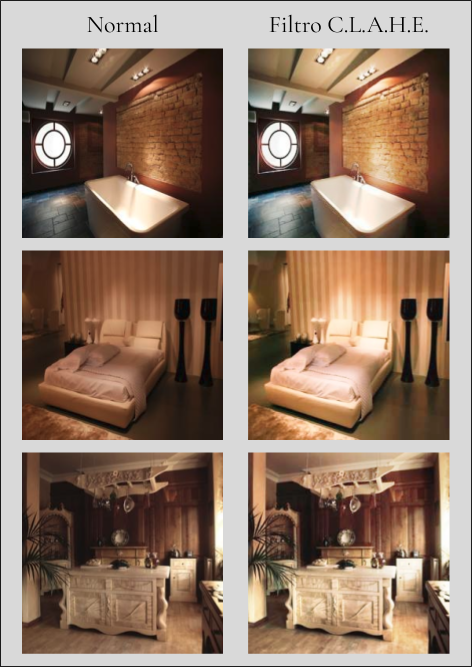
\includegraphics[width=1\linewidth, height=1\textheight]{images/normal_vs_clahe_png}
	\caption[Ejemplo aplicación del algoritmo C.L.A.H.E. en imágenes del dataset utilizado en el experimento \ref{sssec:exp6}]{Ejemplo aplicación del algoritmo C.L.A.H.E. en imágenes del dataset utilizado en el experimento \ref{sssec:exp6}}
	\label{fig:normal_vs_clahe}
\end{figure}

\begin{table}[h!]
	\centering
	\begin{tabular}{| l | r | r |}
		\toprule
		Modelo: Aprendizaje & Exactitud Categórica &  Exactitud Categórica \\
		por Transferencia PlacesCNN & Conj. de Validación &  Conj. de Verificación \\
		\midrule
		Variante 5 & 0.656 & 0.642 \\
		\bottomrule
	\end{tabular}
	\caption{Exactitud categórica para los conjuntos de validación y verificación experimento \ref{sssec:exp6}}
	\label{exp6:results}
\end{table}

En la tabla \ref{exp6:results} se pueden observar los resultados del modelo, con lo cual no existen evidencias suficientes para decir que la hipótesis \ref{sssec:hipotesis6} sea inválida. El hecho de aplicar el filtro C.L.A.H.E. no hizo que los resultados mejoren en gran medida en relación a haber dejado las imágenes en crudo, pero de todos modos el modelo de este experimento obtuvo mejor exactitud categórica que el del experimento \ref{sssec:exp4}.	